
\section{Classified Performance Evaluation of Image-Based VTON}

\subsection{Image-based VTON algorithms}

In this Section, we started with evaluating the 2D image based VTON algorithms using a try-on cloth and a target human image. The human representation is composed of 1) heat maps for each joints 2) silhouette of human body, and 3) face and skin pixels patches (non-cloth and human identity area). It is assumed that the target human image is pre-processed for a cloth agnostic human representation by a human pose estimation like OpenPose\cite{Cao2018OpenPoseRM} and human parsing like LIP \cite{Liang2018LookIP}. 

The previous algorithms are mostly composed of two stages: (1) cloth warping step that warps the try-on cloth to align with the pose and shape of the target model (called GMM in CP-VTON \cite{Wang2018TowardCI}: geometric Manipulation Module), and (2) blending step that blends the warped cloth onto the target human image (called TON in CP-VTON: Try-On Network). 

% the algorithms 
We use the same dataset collected by Han et al. used in VITON\cite{Han2017VITONAI} and CP-VTON\cite{Wang2018TowardCI} papers. Here we include the SCM based-VTON, VITON \cite{Han2017VITONAI}, and  CP-VTON \cite{Wang2018TowardCI}. We included the SCM based algorithm  for a representative of non deep learning algorithm. The cloth warping step is done using SCM matching and transform from try-on cloth to the current, target cloth segmentation area, and the final VTON image is blended using simple alpha blending. For VITON and CP-VTON, a brief suumary is as follows. For more details, the reader is refer to the original papers.
% GMM
The VITON use an encoder-decoder network to generate the warped cloth mask. Then the estimated TPS parameter from SCM matching between the generated mask and input try-on cloth mask is applied to the input try-on cloth. This is because in general the generated images from an encoder-decoder network does not preserved the original cloth as well as the warped image by geometric transform. Instead, CP-VTON uses a CNN based correlation network to estimated the TPS parameter directly and use the estimated parameters for warping.   
% TOM
In the blending step, VITON generates an alpha blending mask image, which is used when alpha-blended with warped try-on cloth and human input image. The authors of CP-VTON observed that the blending is not successful when the warped  cloth area does not align well with the target area of human image, and first generates a coarse VTON results in addition to the composition mask, and then alpha-blends the warped cloth and the coarse VTON image with the alpha-composition mask.        


Differently from other GAN applications where the main purpose is to generate an unseen, plausible image, VTON application needs to retain the original texture and shape of the input try-on cloth. Due to its higher performance and logical architecture, CP-VTON \cite{Wang2018TowardCI} has become the benchmark benchmark algorithm for the image-based VTON algorithms recently published 
% \cite{     }.  But we can not include them in this paper because the implementations are not available. However, we believe the works share the strength and problems with three algorithms examined here. 


%The previous and following in 2019 share same input image and information conditions with CP-VTON and compare the results with it.
% Add some paper summary after CP-VTON .... and explain the differences from our works.

 
\subsection{The Sample Classification Rule}

% The criteria for classification   
First of all, the criteria for classifying the experimental samples were divided into the complexity of try-on cloths and the degree of occlusion (OP, OB, OF), posture (P), and shape (S) of the target cloth area of the human images. For the complexity of try-on cloths, we only uses two groups: long sleeved vs short sleeved, because the length of sleeves is the biggest component in cloth warping and the dataset does not have full styles.    


%The degree of obscuration is a factor that affects the accuracy of the object of deformation, the posture is the degree of deformation, and the complexity of the clothes means the processing complexity of the clothes themselves.
%However, it is included in the range of classification, but not included in the actual experiment is shown in parentheses. Excluded conditions are those that are not included in the test data or that the evaluation is considered to be complex in the current technology. Based on this, six cases were classified as follows.

\begin{itemize}

\item[$\bullet$] B:  no or little occlusion and posture (with long sleeve and  short sleeve)
\item[$\bullet$] OP: the target area partly covered by hair and arms
\item[$\bullet$] OB: A large part of the clothing is covered by the bottoms.
\item[$\bullet$] OF: the target area covered by the arms (with long sleeve and short sleeve)
\item[$\bullet$] P:  large posture deformation (e.g. a large movement of the arm or twisted or lateral posture)
\item[$\bullet$] S:  large body shape change  (over-weighted or pregnant)

\end{itemize}

The cloth shape in the VITON dataset are mostly simple in shape and texture, e.g. a T-shirt (without a collar) of  monochromatic or monotone patterns. Even though it is clearly biased dataset, it is also not easy to define the un-biased one. Although all 2023 test images are used for experiment, some categories, e.g. S, does not have only small samples. But the trends of results in each category are very clear. 


For evaluation of performance, we used same cloth re-try on and new cloth try-on. 
The same cloth re-try-on experiment are done for quantitative evaluation of the algorithm with the ground truth results. 

\subsection{Same Cloth Re-Try-On Result} 

In the same clothing experiment, we evaluate GMM step performance using IoU (intersection over union) and TOM step performance using average SSIM (Structured Similarity Index).

\begin{equation}
 IoU = \frac{ \hat{M}_{warped} \cap M_{cloth}}
            { \hat{M}_{warped} \cup M_{cloth}}
\end{equation} 


\begin{equation}
 SSIM = \frac{ ( 2 \mu_x \mu_y + c_1 )(2 \sigma_{xy} + c_2) }
             { ( \mu^2_x + \mu^2_y +c_1) ( \sigma^2_x + \sigma^2_y + c_2)}
 \end{equation} 

\begin{itemize}

\item[$\bullet$] B: All three algorithms show higher performance for short-sleeve cloth. In particular, SCM-based shows high performance. However, for long arms, the deformation of the arm was not good. This result shows the matching and deformation are mainly done globally based on the whole silhouette, but not optimized for local deformation at sleeve area. TOM stage in VITON and CP-VTON hides some degree of mis-alignment by blending the un-covered target cloth area.   %Including the skeletal information can be supplemented, but at present, no algorithm has been developed for automatically extracting the skeletal information of the garment.

\item[$\bullet$] OP: Partial occlusion by hair and other parts, cause wrong target cloth area and human silhouette. All three algorithms affected this strongly. Therefore, it is expected to improve the GMM part by removing elements such as hair and using only body shapes.

\item[$\bullet$] OB: Occlusion due to bottoms occurs. SCM algorithm does not distinguish between deformation and occlusion and use the target cloth area directly for deformation parameter estimation.  Therefore, GMM results show unnatural deformation especially for long cloths. Since VITON and CP-VITON use silhouette from cloth-agnostic human representation, this effect are reduced.

\item[$\bullet$] OF: TOM of all three algorithms are confused in deciding whether the arm area should covered by cloth or skin color, especially when the new cloth's sleeve length are different from the current cloth's.  

\item[$\bullet$] P: All three algorithms have a big error in the clothing deformation. This is considered to be a big limitation using the two-dimensional algorithm.

\item[$\bullet$] S: In VITON dataset, the matching cloth is large for big human images, the effects is not serious for the same cloth re-try-on.
\end{itemize}

\subsection{ New Cloth Try-On Results }
 
The wearing of a new cloth is, in effect, the ultimate result of the application. As above, objective evaluation is not possible with VITON dataset. Therefore we compare the relative differences of each algorithm based on visual observations.

\begin{itemize}

\item[$\bullet$] B: The clothing deformation itself shows good results similar to the result with same cloths, but there are some differences according to the algorithms in the synthesis. When switching from long to short sleeves, SCM does not restore the skin area, whereas VITON and CP-VTON can generate the skin area for the revealing bare arm. Especially due to the coarse VTON output of it, CP-VTON can generate much clear skin area.

\item[$\bullet$] OP: The performance was similar to that of the same clothes.

\item[$\bullet$] OB: The same characteristics as the same image, that is, the SCM shows a problem that can not distinguish between the mask and deformation.

\item[$\bullet$] OF: The same characteristics as the costume. Here too, in the case of SCM, the synthesis algorithm needs to be improved when switching from short arm to long arm.

\item[$\bullet$] P: As in the case of the same costume, there was a large error in deformation.

\item[$\bullet$] S: Results shows GMM, especially of VITON and CP-VTON, can warp the new cloth to the target human body shape change, 

\end{itemize}

%In addition to the analysis of each condition in addition to the analysis of each condition, it can be seen that there are the following big features. First, it was confirmed that the shape change of clothes by GMM has an influence on the current wear clothes. The reason is that SCMM uses the area of the current costume, and deep learning methods use the body itself, but the area of the current costume is reflected in the correct answer mask used in the learning process.

 
\subsection{Discussion for Improvement}

% comparison between algorithm
Comparing the performance the algorithms used, CP-VTON show the best quality in both same cloth re-try-on and new cloth try-on. However there are some notable observations. CP-VTON GMM using CNN Geometry matching algorithm shows better results than VITON GMM. The GMM results for the same cloth shows SCM show best quality, which might sound conflicting against the result in \cite{Wang2018TowardCI}. It can be explained that only new cloth case are examined in \cite{Wang2018TowardCI}. whereas SCM can use the ground truth target in same cloth re-try-on.  In the same cloth re-try on, SCM show more reliable results than the current CNN Geometry matching algorithm used in CV-VTON.       
As for TOM stage, VITON generates blurred cloth due to the un-clear composition alpha-map, CP-VTON generated much clear cloth texture, and SCM generates noticeable cloth boundary.     


%All the used image-based algorithms shows similar trends in each input
%Even though the success and failure cases are presented and compared with other algorithms' results, the failure case analysis is not enough for understanding the origin of failure cases and therefore difficult to find the solution for them. A classified evaluation would be better for this understanding. Here we summarized the classified results from our another study. We classify input try-on cloth and target human images according to the posture and body type of the person, the degree of occlusion of the clothes, and the characteristics of the clothes. Quality is compared in IoU for the warping step and in SSIM for the final blending step for same cloth re-try-on cases. We also tested for the new cloth try-on cases but did not include here for limitation of spaces, and the same cloth cases are enough to explain the tendencies of the performances. Though in general CP-VTON generates the best quality image, the relative comparison is not the main purpose of the analysis. Please refer to Figure \ref{fig:classified2DVTONresult} for detailed results.


\begin{figure}
\centering
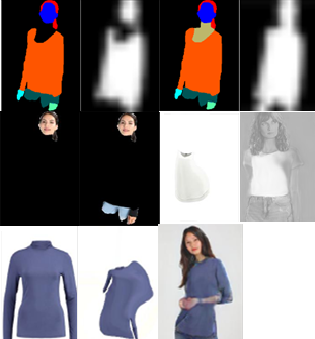
\includegraphics[height=8.5cm, scale=1]{figures/cpvtonissues.png}   % TODO
\caption{The issues in CP-VTON}
\label{fig:cpvtonissues}
\end{figure}

% 1.
Firstly, even though they argued and tried to use cloth-agnostic human representation, the current VITON target try-on area is dependent upon current cloth shape. Especially, the neck area pixels are labeled as background and some body areas are occluded by hairs or accessories (Figure \ref{fig:cpvtonissues}), which affects in cloth warping and blending. 
% 2.
Secondly, all the unintended part, faces, bottom-clothes and legs have to be preserved in blending stage. But other parts except face and hair are missing in CP-VTON\cite{Wang2018TowardCI} human representation and generated at blending stage, which is all right for general synthesis application but not desirable in VTON application (Figure \ref{fig:cpvtonissues}). 
% 3.
Thirdly, the texture is often not vivid, which is due to the composition. Examining the original loss function of TOM network, the term for the composition alpha mask are poorly formulated as simple regularization loss.   

\begin{equation}
L = c_1 | I_0-I_{GT} |+  c_2 L_{VGG}+c_3 |1-M_0 |        
\end{equation} 

%4. 
Fourthly, since no label in the area of warped cloth is the same color as background, white colored clothes are confused and improperly processed in the blending stage (Fig. 3 (c))


Finally, GMM module using Spatial Transform Network\cite{JaderbergSZK15} with TPS (Thin Plate Spline)\cite{Bookstein1989PrincipalWT} deformation cannot handle strong 3D deformation due to the target pose and also generates artifacts because of the person representation inputs. For example, hands-up and folded arms.  Note that many errors in the warping stage are often hidden in the blending stage when the target clothes are single-colored, which can be expected in practical conditions 
%(Fig. 3 (d)).


%Especially note that the warped cloth are often too much different for desired shape. It is originated two facts. First the 3D deformation that any 2D deformation including non-rigid transform such as TPS is quite limited, especially any 2D deformation cannot handle when the two area in the original image are overlapped in the destination images. There for when the arms of long sleeved cloth occlude the main body, 2D warping cannot approximate the 3D deformation properly. Second, the deformation needs corresponding points  between the source nd target image. The cloth are extremely difficult object to find the corresponding points. The STN (spatial transform network)\cite{JaderbergSZK15} and SCM (shape context matching)\cite{BelongieMP02} cannot find the corresponding points when the target cloth and original cloth has different shapes. In conclusion, the 2D image based algorithm has serious limitation in the range of applications. It can apply to the mild posed target human only and simple short sleeved cloth, mainly because the inherent limitation of 2D deformation method including non-rigid ones, and the poor performance of matching algorithm.  To overcome this limitation, we consider to model the try-on cloth into 3D model and apply the 3D deformation

\begin{figure}
\centering
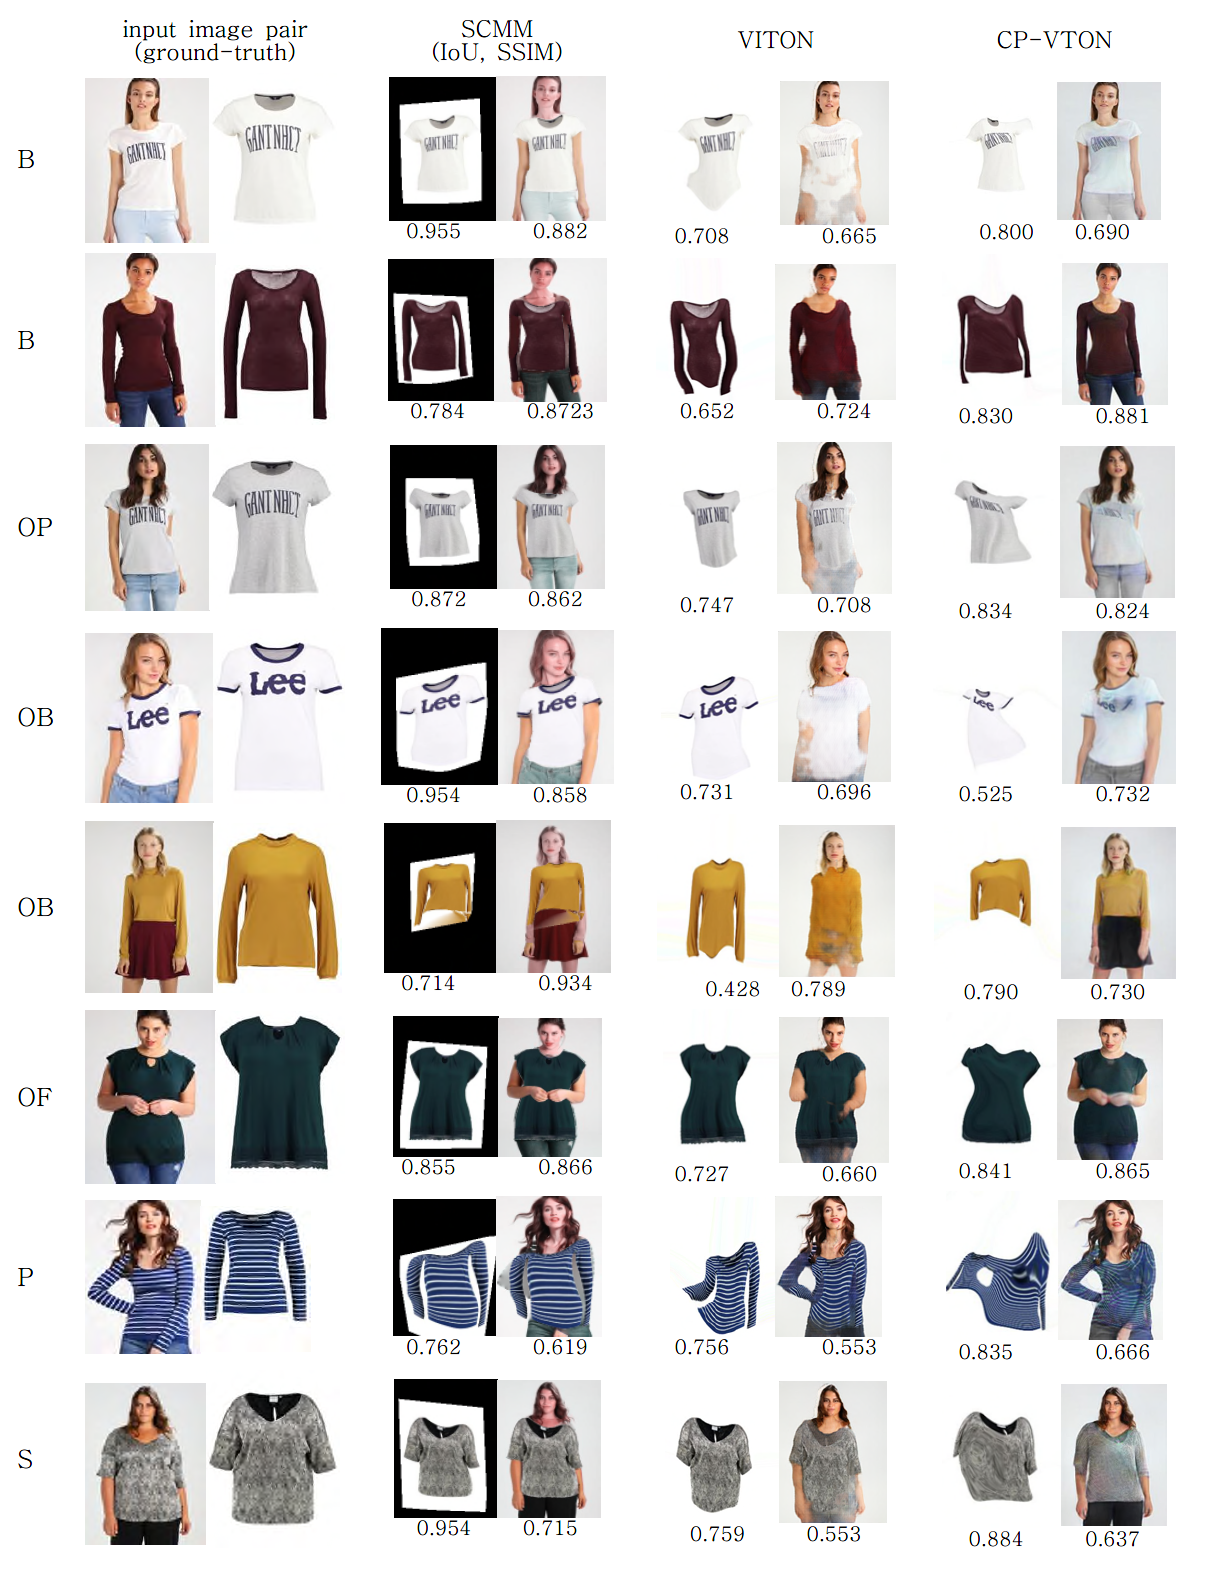
\includegraphics[height=13.5cm, scale=1]{figures/2dvton_same.png}   
\caption{Classified Evaluation of Image-based VTONs (same cloth re-try-on)}
\label{fig:2dvton_same}
\end{figure}

\begin{figure}
\centering
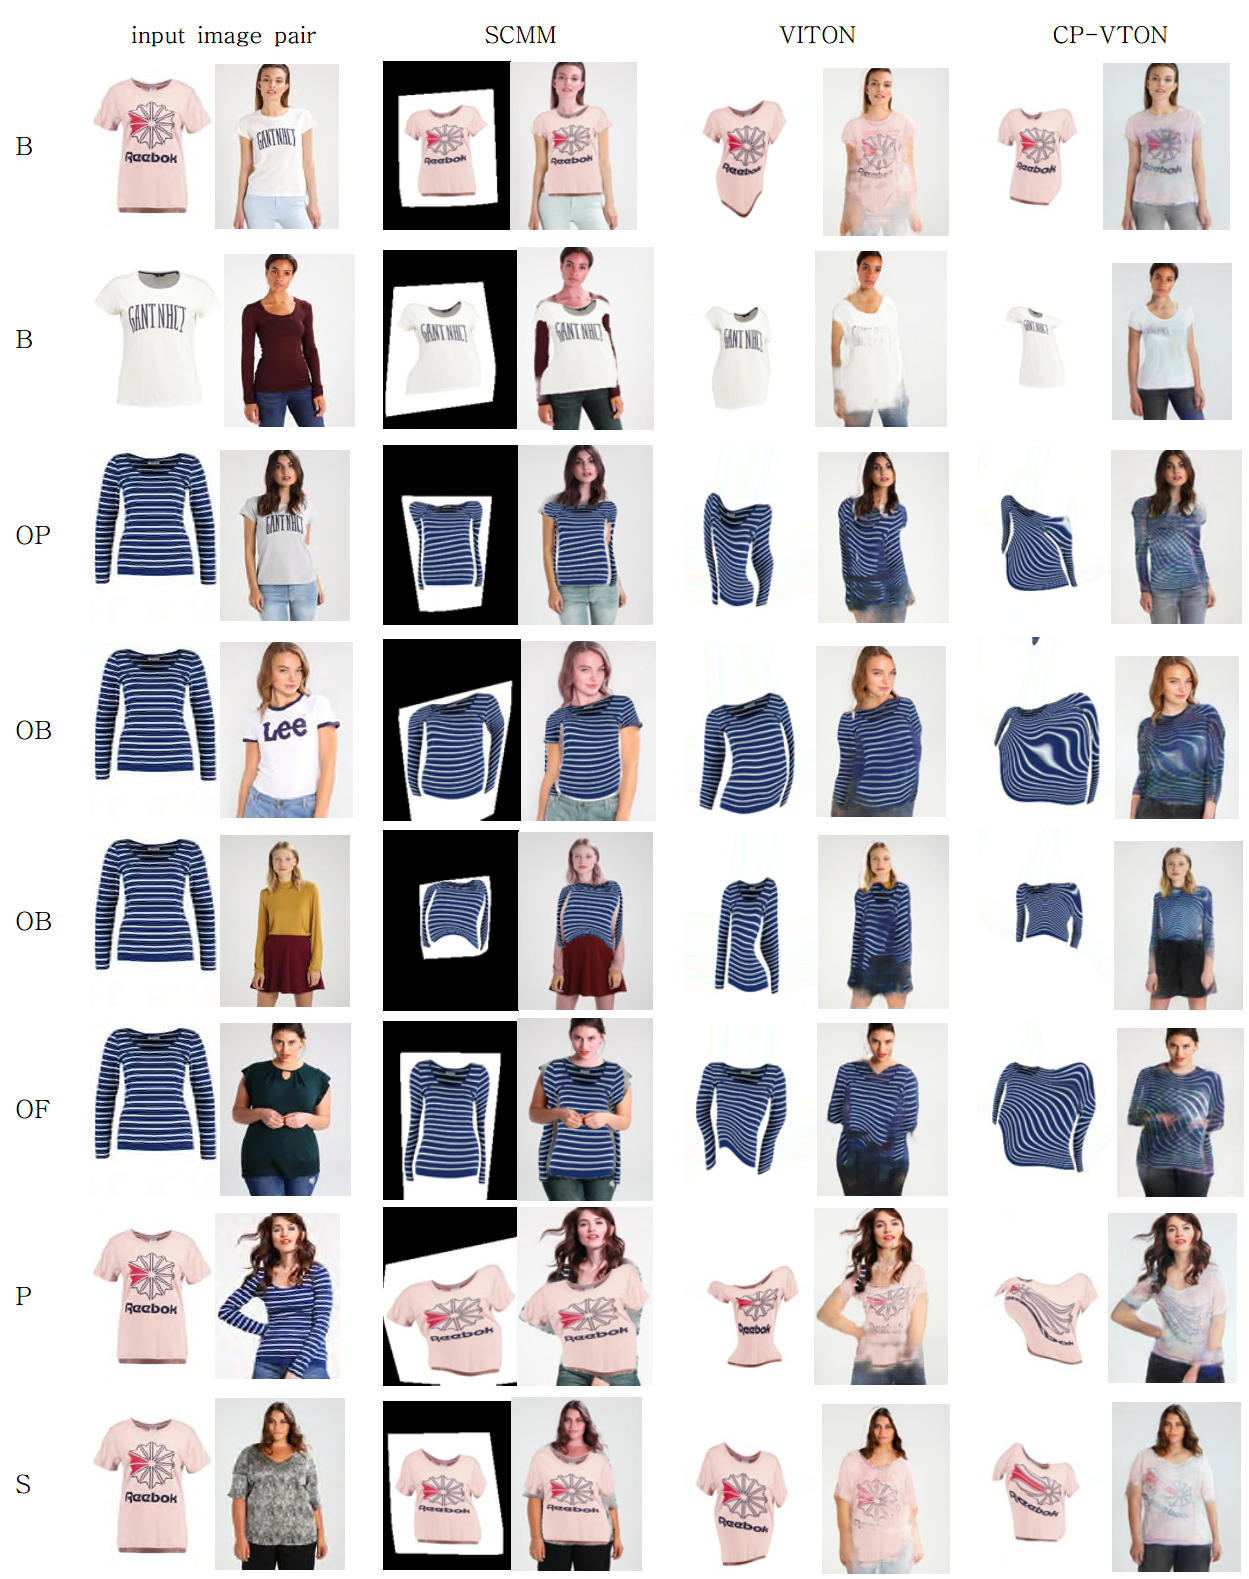
\includegraphics[height=13.5cm, scale=1]{figures/2dvton_diff.png}  %% TODO  
\caption{Classified Evaluation of Image-based VTONs (new cloth try-on)}
\label{fig:2dvton_diff}
\end{figure}
